\chapter*{Anexo}
\addcontentsline{toc}{chapter}{Anexo}
El presente capítulo es de utilidad para aquellos que pretender modificar o extender el \emph{framework} propuesto en este informe. El proyecto se puede clonar desde el repositorio de \texttt{GitHub} \href{https://github.com/rgaluppo/runtime_permissions_test}{runtime-permissions-test}. Al ser una aplicación híbrida que utiliza \emph{plugins} de Apache Cordova, es requisito indispensable instalarlo.\\

A continuación se presentan los pasos para instalar el proyecto, arrancado desde cero; su estructura y una guía para agregar tests.
\section*{Pasos para instalar el proyecto}
\begin{enumerate}
    \item Instalar Apache Cordova.
        \begin{lstlisting}[style=DOS]
  user $> npm install -g cordova
        \end{lstlisting}
    \item Clonar el proyecto \href{https://github.com/rgaluppo/runtime_permissions_test}{runtime-permissions-test}.
    \begin{lstlisting}[style=DOS]
  user $> https://github.com/rgaluppo/runtime_permissions_test.git
  \end{lstlisting}
    \item Agregar plataforma según corresponda.
        \begin{lstlisting}[style=DOS]
  user $> cordova platform add ios
        \end{lstlisting}\\
        \begin{lstlisting}[style=DOS]
  user $> cordova platform add android
        \end{lstlisting}
    \item Agregar \emph{plugins} de Apache Cordova.
        \begin{lstlisting}[style=DOS]
  user $> cordova plugin add cordova.plugins.diagnostic@3.0
  user $> cordova plugin add cordova-plugin-calendar
  user $> cordova plugin add cordova-plugin-contacts
  user $> cordova plugin add cordova-plugin-geolocation
  user $> cordova plugin add cordova-sms-plugin
  user $> cordova plugin add https://github.com/gitawego/cordova-screenshot.git
  user $> cordova plugin add cordova-plugin-device
  user $> cordova plugin add cordova-plugin-device-motion
  user $> cordova plugin add cordova-plugin-gyroscope@0.1.4
        \end{lstlisting}
    \item Correr la máquina virtual según la plataforma elegida.
        \begin{lstlisting}[style=DOS]
  user $> cordova emulate ios
        \end{lstlisting}\\
        \begin{lstlisting}[style=DOS]
  user $> cordova emulate android
        \end{lstlisting}
\end{enumerate}
\section*{Extensión del Framework}
El \emph{framework} propuesto en el capítulo 6 es una aplicación híbrida, desarrollada utilizando Apache Cordova. Para acceder a funciones del teléfono, hay que agregar distintos \emph{plugins}. Algunos de ellos fueron desarrollados por Apache Cordova, mientras que el resto fueron desarrollados por usuarios. Independientemente de su creador, un \emph{plugin} puede descargarse a través de \texttt{npm} o un repositorio \texttt{git}.\\

\begin{figure}[hbtp]
    \centering
	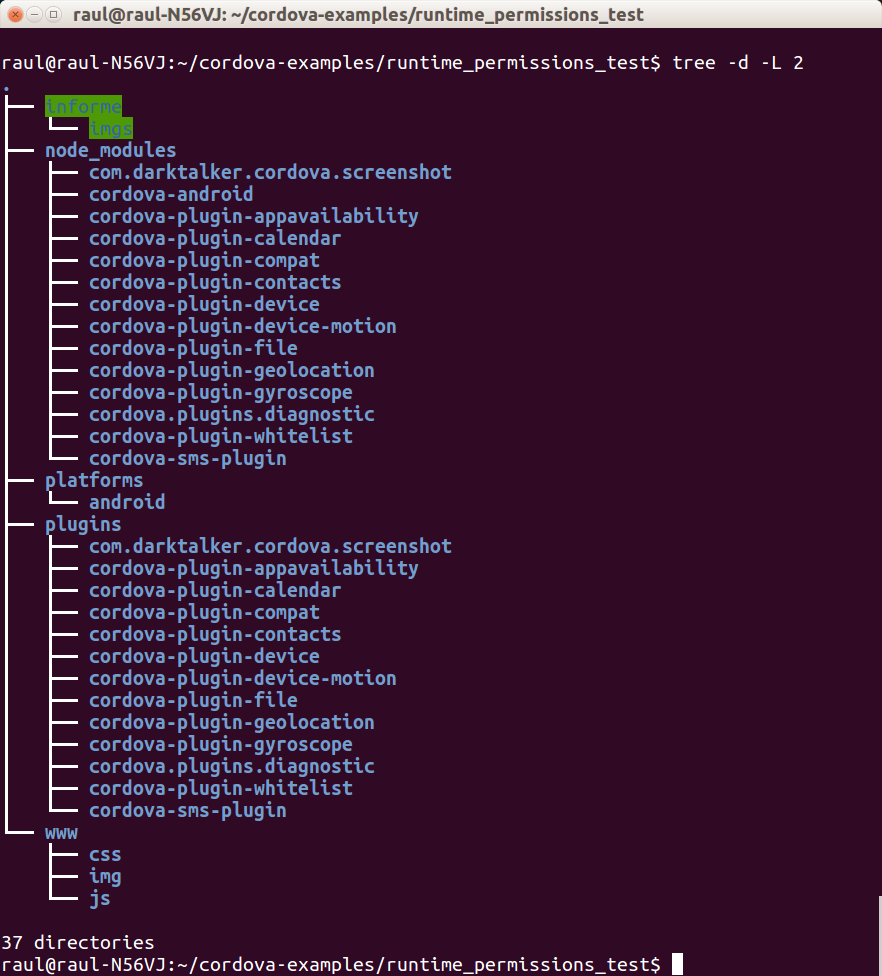
\includegraphics[width=.85\linewidth]{anexo/cordova-files-struct}
	\caption{Estructura de archivos de un proyecto Apache Cordova.}
    \label{fig:anexo:cordova-files-struct}
\end{figure}
Cada proyecto de Apache Cordova tiene una estructura particular, como se observa en la Figura \ref{fig:anexo:cordova-files-struct}. Se pueden destacar tres carpetas:
\begin{itemize}
\item \texttt{platforms}: contiene las plataformas agregadas al proyecto.
\item \texttt{plugins}: contiene los \emph{plugins} agregados al proyecto.
\item \texttt{www}: contiene todos los recursos que utiliza la aplicación híbrida.
\end{itemize}
Al ser el \emph{framework} una aplicación híbrida, dentro de la carpeta \texttt{www} se encuentra una estructura típica de una pagina web. En ella se encuentra el archivo \texttt{index.html}, junto con los recursos necesarios. En caso de requerirse alguna librería de Javascript, debería estar dentro de esta carpeta.\\

Para el caso particular del \emph{framework} propuesto, se creó la estructura de archivos que se observa en la Figura \ref{fig:anexo:framework-files-struct}. En el archivo \texttt{index.html} se encuentra el diseño de la aplicación. En la carpeta \emph{js} se encuentran varios \emph{scripts}. Hay uno responsable de interactuar con el usuario, mientras que el resto de los \emph{scripts} contiene un test concreto, los cuales fueron explicados en el capítulo 6.\\
\begin{figure}[htbp]
    \centering
	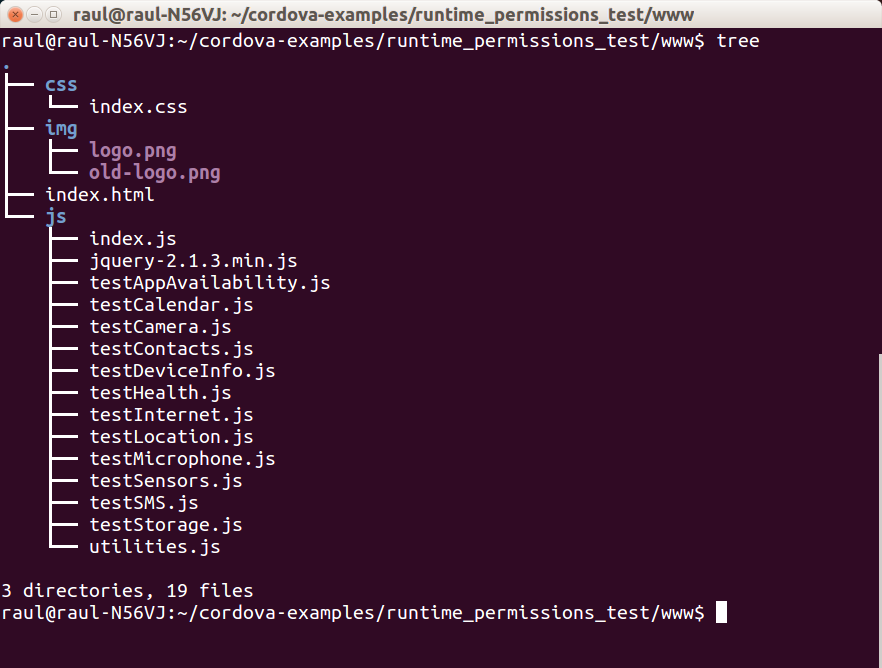
\includegraphics[width=\linewidth]{anexo/framework-files-struct}
	\caption{Estructura típica de una aplicación híbrida.}
    \label{fig:anexo:framework-files-struct}
\end{figure}

A continuación, se detallarán una serie de pasos que servirán de guía a la hora de extender el \emph{framework}:
\begin{enumerate}
\item Pensar un test.
\item Determinar el componente a testear.
\item Buscar \emph{plugins} de Cordova que permitan acceder a las funcionalidades del componente deseado.
\item Desarrollar un \emph{script} de JavaScript que implemente la lógica del test, realizando invocaciones a los \emph{plugins}.
\item Agregar al archivo \texttt{index.html} un gesto para interactuar con el usuario (un botón, por ejemplo).
\item Implementar la interacción deseada en el archivo \texttt{index.js}.
\end{enumerate}